\chapter{Introduction \& Literature Review}
\thispagestyle{empty}

\section{Galaxy Evolution}
\subsection{Large Scale Structure}
Approximately $10^{-33}$ seconds after The Big Bang, the universe began to expand due to the negative pressure of dark energy \citep{linde_new_1982, frieman_dark_2008, baumann_tasi_2009, desi_collaboration_desi_2024}. Gravitational instabilities in the early universe arose from quantum fluctuations in the hot, dense plasma of baryonic matter that magnified due to the expansion of the universe \citep{bond_how_1996, beutler_6df_2011, desi_collaboration_desi_2016}. These tiny perturbations in the matter density from the early universe ($z>1,000$; \citealp{beutler_6df_2011}) have become known as \gls{bao}, where the tight radiative pressure of the compacted universe gives rise to sound waves emanating from over-dense clustering regions \citep{eisenstein_baryonic_1998, eisenstein_detection_2005}.

As the universe expanded at an accelerating rate, adiabatic cooling took place. The once-dense plasma medium could no longer sustain further \gls{bao} ($z<1,000$; \citealp{eisenstein_detection_2005, baumann_tasi_2009}). The quantum fluctuations were then preserved in what is now known as the \gls{cmb} \citep{eisenstein_baryonic_1998, planck_collaboration_planck_2020-1}, approximately $380,000$ years after The Big Bang. \Cref{Fig: CMB} illustrates the small temperature variations in the \gls{cmb} detected by the \textit{Planck} mission \citep{planck_collaboration_planck_2020}. The first high-precision detection of these fluctuations was achieved by the \gls{wmap} team in 2003 \citep{spergel_first-year_2003} followed by numerous subsequent studies \citep{hinshaw_nine-year_2013}. Most astrophysical research relies on the above cosmological framework, known as \gls{lcdm} cosmology. Also often referred to as the ``standard cosmological model", it posits that the universe is spatially flat and consists of approximately 5\% baryonic matter, 25\% dark matter, and 70\% dark energy \citep{desi_collaboration_desi_2024}. This framework forms the \gls{lcdm} model, where $\Lambda$ is Einstein's cosmological constant \citep{einstein_kosmologische_1917}, signifying the dominant contribution of dark energy.

\begin{figure}
    \centering
    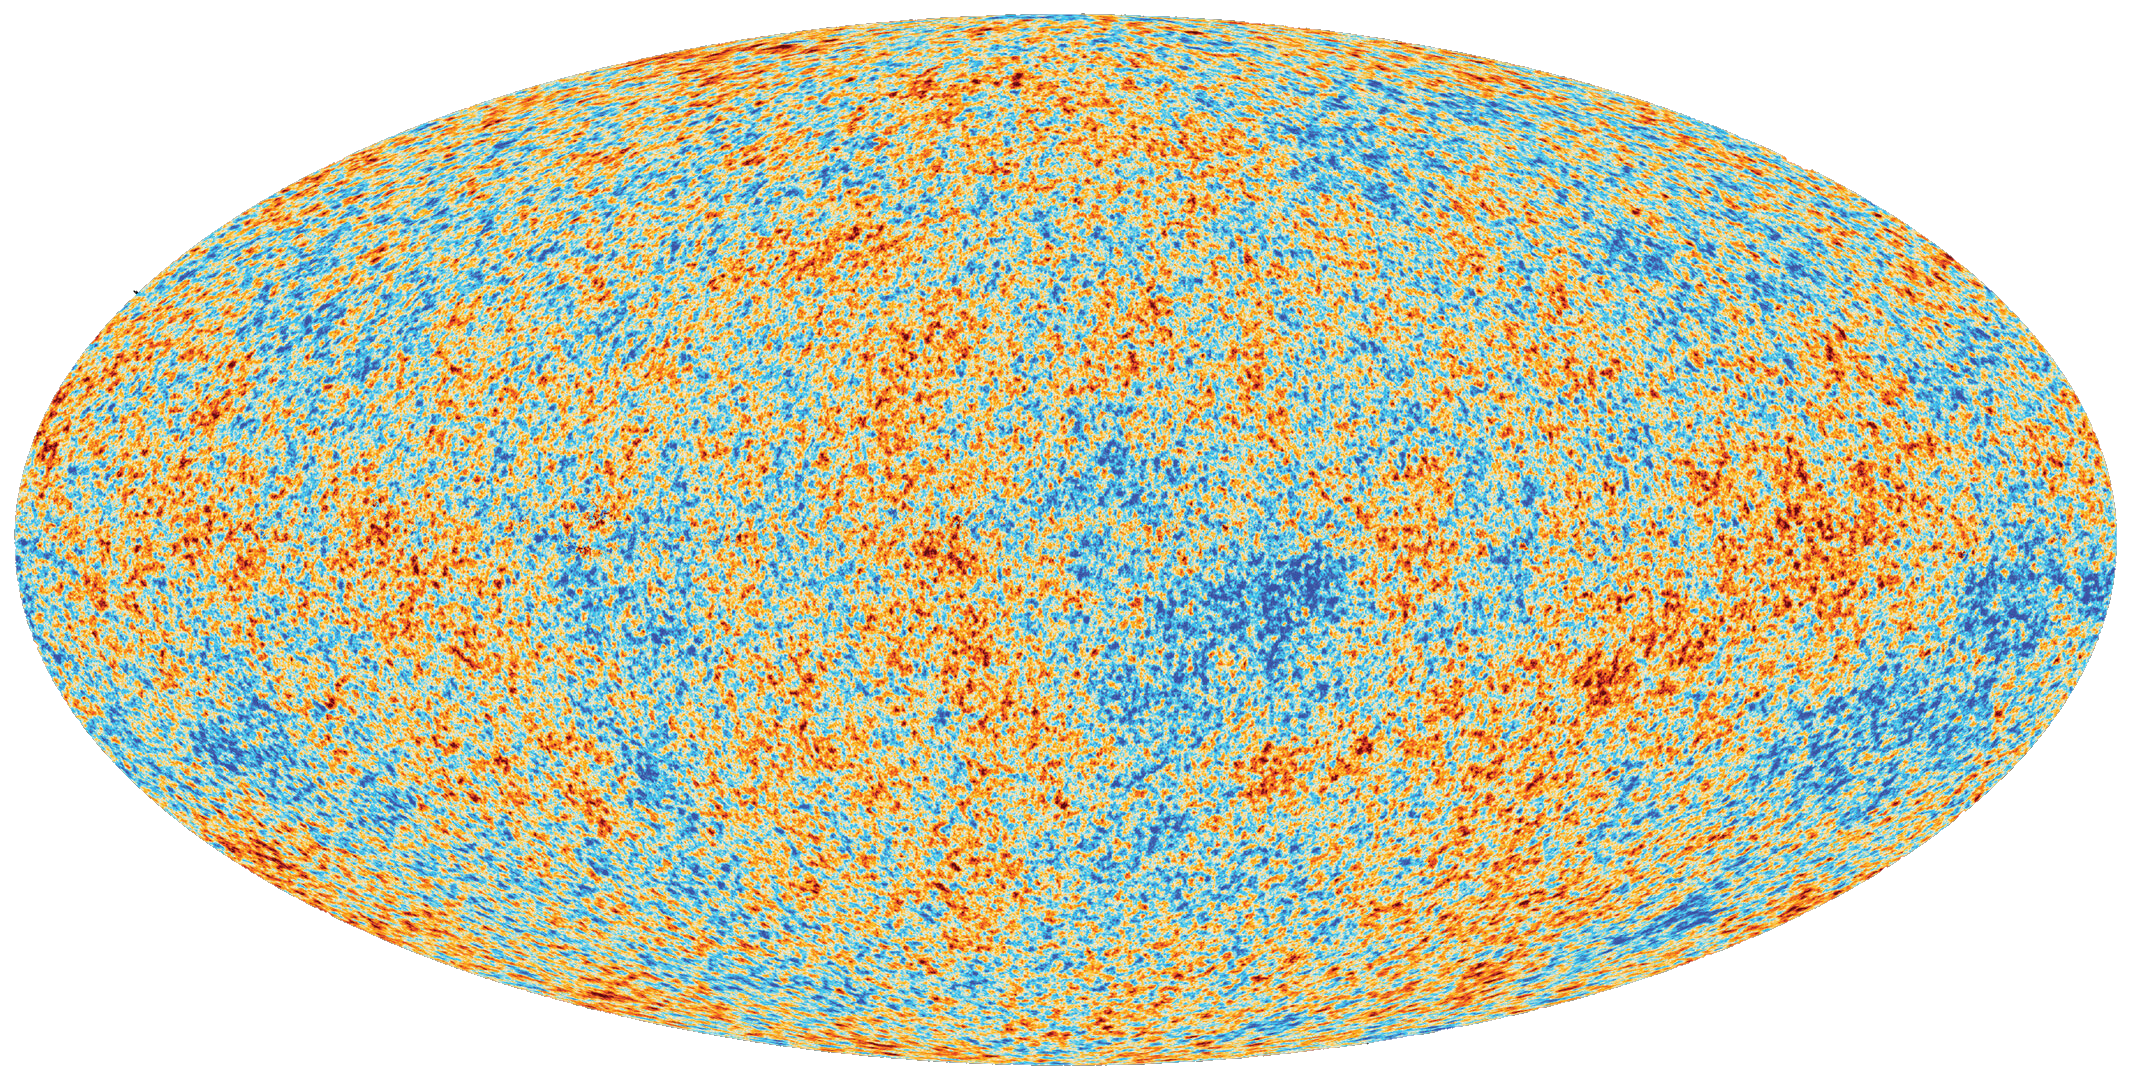
\includegraphics[width=\textwidth]{Figures/CMB.png}
    \caption{Anisotropies in the Cosmic Microwave Background from the 2018 Planck Legacy data release \citep{planck_collaboration_planck_2020}.}
    \label{Fig: CMB}
\end{figure}

When we think of our place in the universe, we often think in a hierarchical order akin to \textit{City, Country, Earth, Sol System}. But this can be extended further to \textit{The Milky Way, The Local Group, Virgo Supercluster, Laniakea Supercluster}, and ultimately the observable universe itself. Each of these nested structures represents a larger scale of cosmic architecture, the growing magnitude of which we can never possibly begin to comprehend. The vastness and complexity of these ``layers" reveal a far more interconnected and dynamic universe than we might initially perceive. In this view, Earth becomes just a tiny dot in a sea of countless galaxies and stars, all governed by the same fundamental forces of nature. 

Referred to as \gls{lss}, the distribution of matter---such as galaxies and black holes---is \textit{not} random \citep{bond_how_1996, coil_large-scale_2013}. On cosmic scales exceeding 100 megaparsecs (Mpc), the universe is generally assumed to be homogeneous and isotropic \citep{friedmann_uber_1922, lemaitre_univers_1927, arjona_complementary_2021, dome_cosmic_2023}. This is known as the cosmological principle and is a core component underpinning all of cosmology \citep{yadav_testing_2005, sarkar_scale_2009, planck_collaboration_planck_2016, planck_collaboration_planck_2020-1, planck_collaboration_planck_2020-2}. In this context, homogeneity means that the distribution of matter is consistent throughout the universe. At the same time, isotropy indicates that the universe appears the same in all directions, with no unique locations or orientations. However, on scales smaller than 100 Mpc, the universe exhibits inhomogeneity and anisotropy, characterised by smaller structures such as galaxies and galaxy clusters. \textcolor{red}{Given the cosmological principle, which posits a homogeneous and isotropic universe on large scales, we can better understand how matter has evolved into the large-scale structures observed today, such as galaxies, clusters, and voids}

\begin{figure}
    \centering
    \includegraphics[width=\linewidth]{Figures/galaxy_distribution.png}
    \caption{The Millennium Run Simulation by \cite{springel_simulations_2005} showcasing the distribution of galaxies connected via a cosmic web of dark matter.}
    \label{Fig: Galaxy Distribution}
\end{figure}

In \cref{Fig: Galaxy Distribution}, the \gls{lss} of the universe can be seen. Voids are stretches of space containing little to no galaxies. Surrounding these low-density environments are galactic filaments, which are ``cosmic highways" that connect over-dense regions containing large clusters of galaxies \citep{darvish_cosmic_2014, okane_effect_2024}. The red areas in \cref{Fig: CMB} indicate overdensities that will form future large structures, while the blue regions will evolve into cosmic voids.

The assumption that the universe is homogeneous and isotropic on large scales suggests that our observations and measurements could be conducted from any location within the universe \citep{clarkson_general_2008}. Despite this, numerous studies have tested the cosmological principle. For instance, measurements of the Hubble constant $H_0$, which indicates the rate of the universe's expansion, should align if the universe is indeed homogeneous and isotropic on large scales. However, research conducted by the Planck Collaboration \citep{planck_collaboration_planck_2020-1} and the SH0ES Team \citep{riess_comprehensive_2022} reveals a $5\sigma$ discrepancy in their determinations of $H_0$. This significant difference could suggest that the universe is not homogeneous and isotropic on large scales \citep{hu_testing_2024}. While the various cosmological implications stemming from these findings are beyond the focus of this thesis's review, the prevailing tension is noteworthy and merits inclusion. In the context of this work, however, the perspective taken is that the universe remains homogeneous and isotropic on large scales.

The distribution of galaxies is distinctly non-random, and the fundamental physics at the beginning of cosmic time has significantly influenced the universe's evolution over the past 13.7 billion years. The \gls{cmb} and \gls{lss} serve as crucial probes, enabling us to directly comprehend the nature of the universe when it was less than one million years old (Myrs). To fully grasp how the universe has evolved to its present state, additional probes are necessary to understand the evolution of structure across cosmic time.